\section{Model 2: Transfer Learning with EfficientNet-B0}

\subsection{Methods}

Model 2 applies transfer learning and is evaluated with two pretrained backbones;
this section describes the first, EfficientNet-B0. In contrast to
the scratch CNN, this model is not initialized randomly. Instead, the
convolutional feature extractor is loaded with ImageNet-pretrained weights
\cite{tan2019efficientnet}. The original ImageNet classifier is replaced by a
new linear classification head with either ten outputs for the original
EuroSAT task or two outputs for the binary vegetation task.

EfficientNet-B0 was selected because it is a compact pretrained CNN and is
therefore suitable for a comparison with the smaller scratch model. Its main
advantage is that low-level and mid-level visual features such as edges,
textures, and object-like patterns are already represented in the pretrained
feature extractor. The model therefore does not need to learn all image
representations from the EuroSAT training split alone.

The input images are resized to $224 \times 224$ pixels, because this is the
standard input size of the ImageNet-pretrained EfficientNet-B0 model in
Torchvision. During training, horizontal flips, vertical flips, and rotations up
to 15 degrees are applied. Validation and test images are not randomly
augmented. All images are normalized with the standard ImageNet mean and
standard deviation, because the pretrained weights were trained with this
normalization scheme.

\begin{table}[H]
\centering
\caption{EfficientNet-B0 transfer learning setup.}
\label{tab:efficientnet_setup}
\small
\begin{tabularx}{\textwidth}{lX}
\toprule
Component & Configuration \\
\midrule
Base model & EfficientNet-B0 with ImageNet-pretrained weights \\
Input & RGB image resized to $3 \times 224 \times 224$ \\
Classifier & Replaced linear layer with 10 or 2 outputs \\
Loss function & \texttt{CrossEntropyLoss} \\
Optimizer & AdamW \\
Batch size & 64 \\
Epochs & 50 \\
Frozen phase & Epochs 1--5: train classifier head only \\
Fine-tuning phase & Epochs 6--50: unfreeze final two EfficientNet feature blocks \\
Model selection & Checkpoint with lowest validation loss \\
\bottomrule
\end{tabularx}
\end{table}

\subsection{Experimental Design}

The same stratified train/validation/test split as for Model 1 was used. This
keeps the comparison between the scratch CNN and the transfer learning model
fair. The two tasks are also identical: the 10-class EuroSAT classification and
the binary vegetation classification.

The training was performed in two stages. First, the EfficientNet feature
extractor was frozen and only the new classifier head was trained. This makes
the new output layer adapt to the EuroSAT labels without immediately changing
the pretrained feature representation. After five epochs, the final two feature
blocks of EfficientNet-B0 were unfrozen and fine-tuned with a smaller backbone
learning rate. This allows the model to adapt its higher-level features to the
satellite image domain.

The final hyperparameters were:

\begin{itemize}
  \item head learning rate: 0.001,
  \item backbone learning rate: 0.0001,
  \item weight decay: 0.0001,
  \item batch size: 64,
  \item seed: 42.
\end{itemize}

The test split was evaluated only after training, using the checkpoint with the
lowest validation loss.

\subsection{Results}

Table \ref{tab:efficientnet_results} summarizes the final EfficientNet-B0
results. For the 10-class task, the best checkpoint was selected after epoch 46.
For the binary task, the best checkpoint was selected after epoch 29.

\begin{table}[H]
\centering
\caption{Final results of the EfficientNet-B0 transfer learning model.}
\label{tab:efficientnet_results}
\small
\begin{tabular}{llrrr}
\toprule
Task & Split & Loss & Accuracy & Macro-F1 \\
\midrule
10-class & Validation & 0.0700 & 0.9793 & 0.9784 \\
10-class & Test & 0.0833 & 0.9726 & 0.9719 \\
Binary & Validation & 0.0130 & 0.9961 & 0.9961 \\
Binary & Test & 0.0184 & 0.9941 & 0.9941 \\
\bottomrule
\end{tabular}
\end{table}

Figure~\ref{fig:efficientnet_multiclass_curves} shows the loss and accuracy curves for the 10-class EfficientNet-B0 model. The strongest improvement occurs after switching from the frozen classifier-head phase to fine-tuning. The best checkpoint was selected in epoch 46 based on the lowest validation loss.

\begin{figure}[H]
    \centering
    \begin{minipage}{0.48\textwidth}
        \centering
        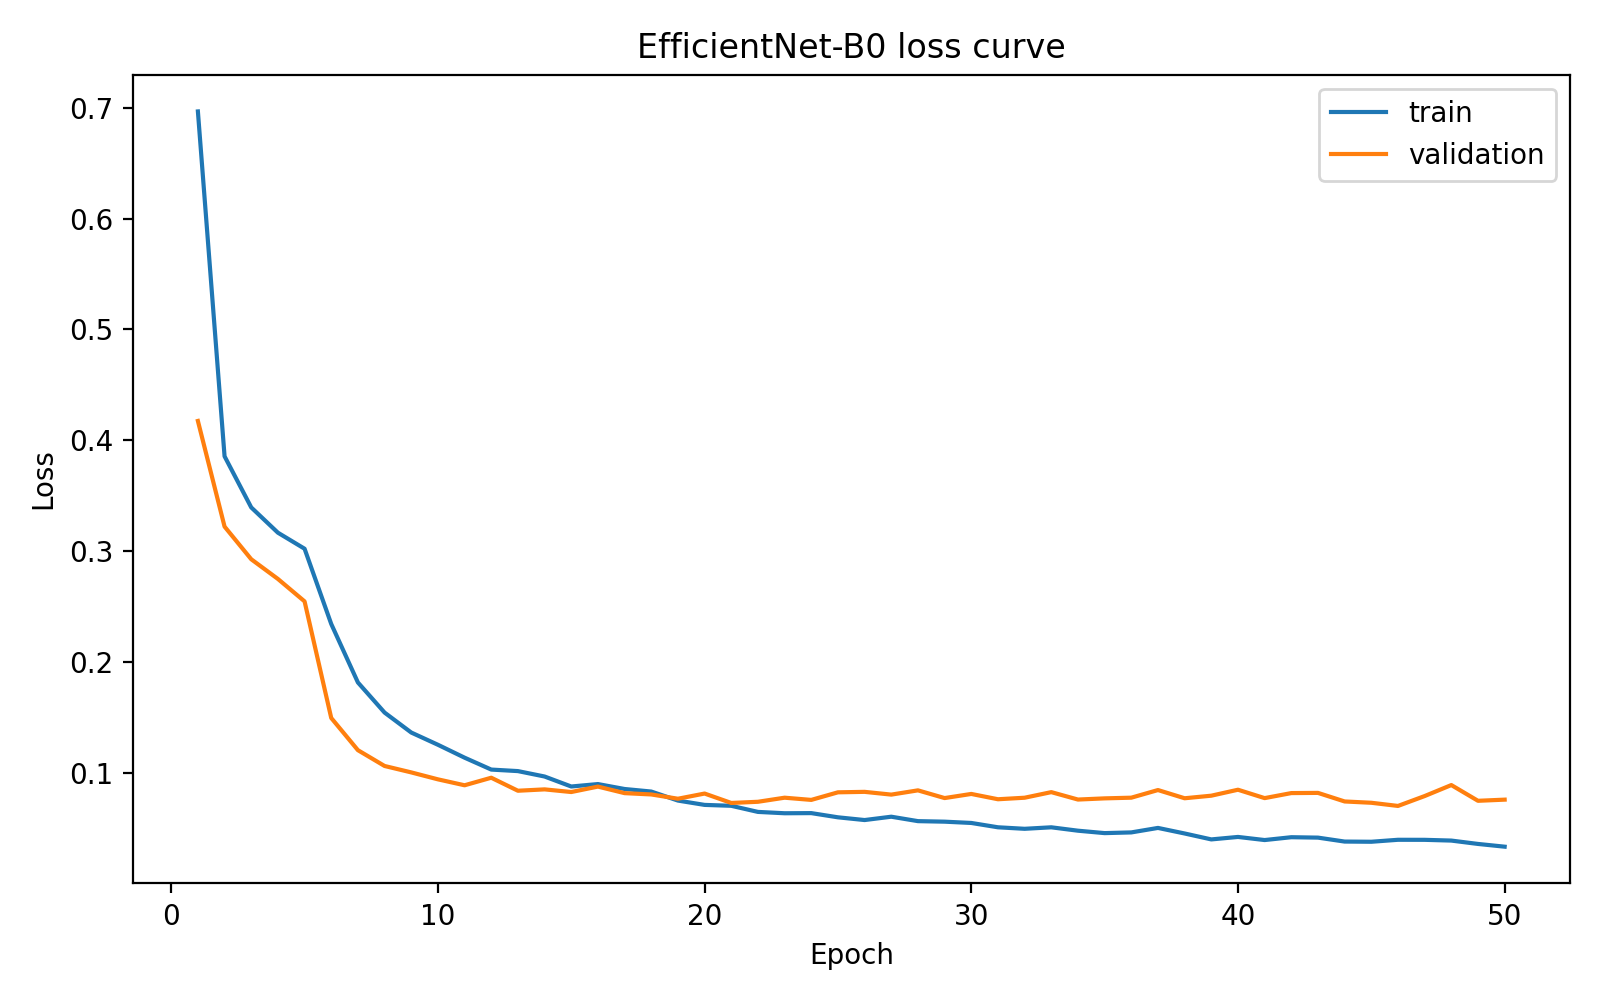
\includegraphics[width=\linewidth]{figures/efficientnet_b0/multiclass_loss_curve.png}
    \end{minipage}
    \hfill
    \begin{minipage}{0.48\textwidth}
        \centering
        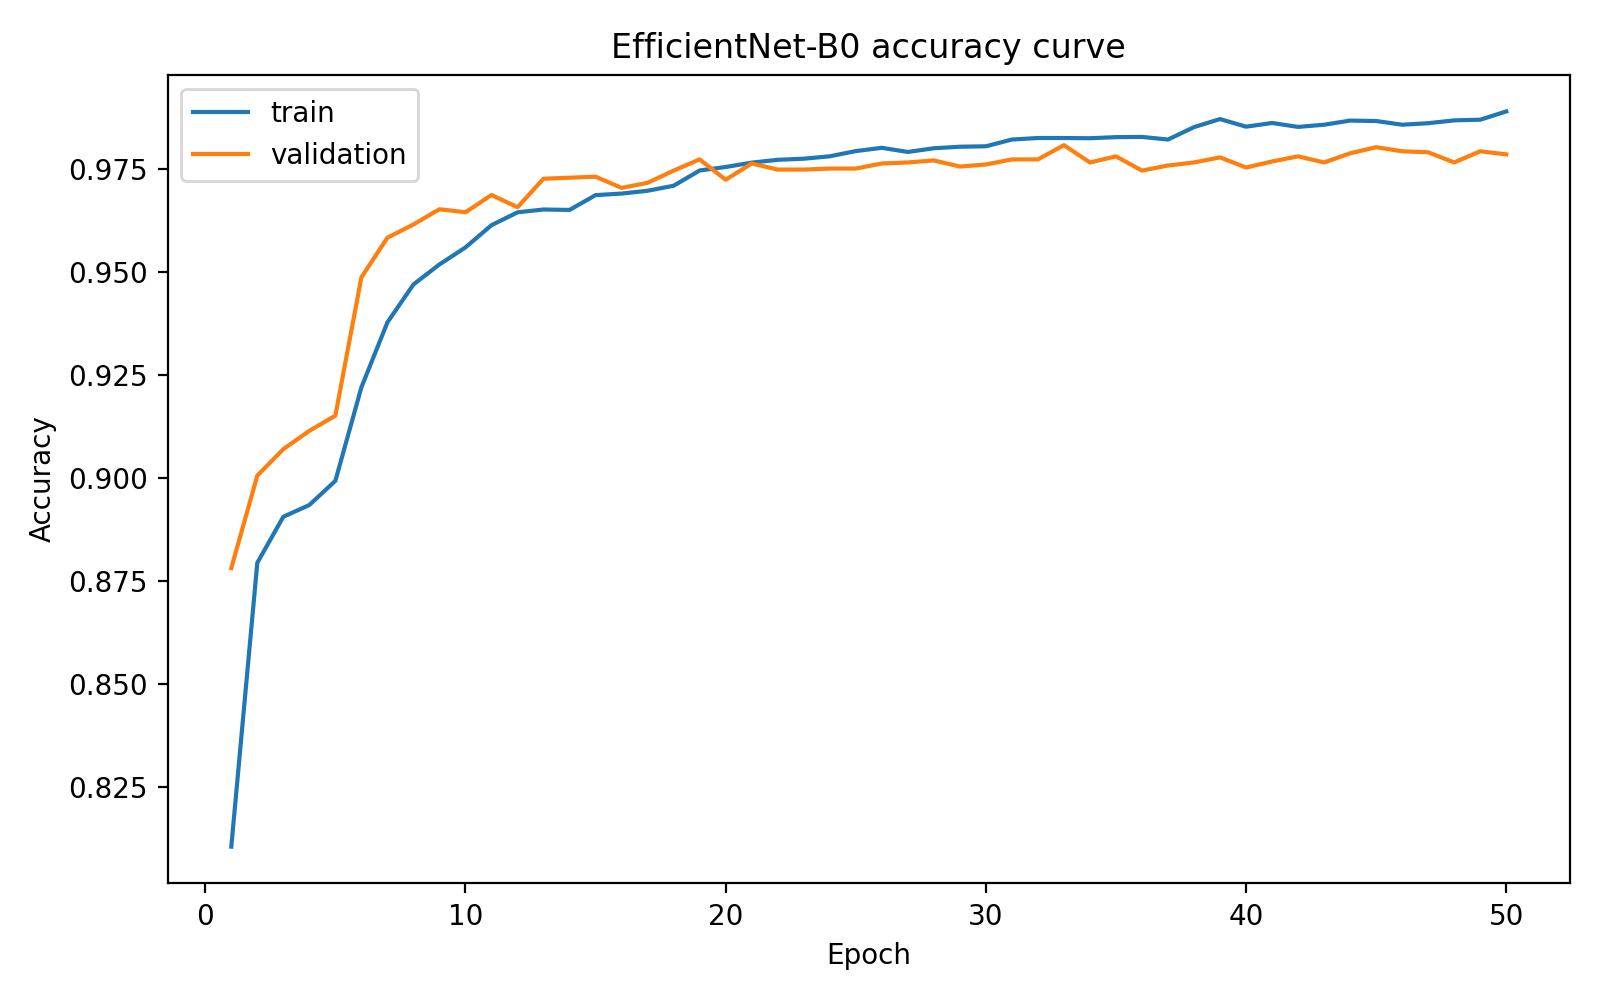
\includegraphics[width=\linewidth]{figures/efficientnet_b0/multiclass_accuracy_curve.png}
    \end{minipage}
    \caption{Loss and accuracy curves of the EfficientNet-B0 model on the 10-class task.}
    \label{fig:efficientnet_multiclass_curves}
\end{figure}

Figure~\ref{fig:efficientnet_multiclass_cm} shows the confusion matrix for the 10-class test split. The remaining errors mainly occur between visually similar land-use classes.

\begin{figure}[H]
    \centering
    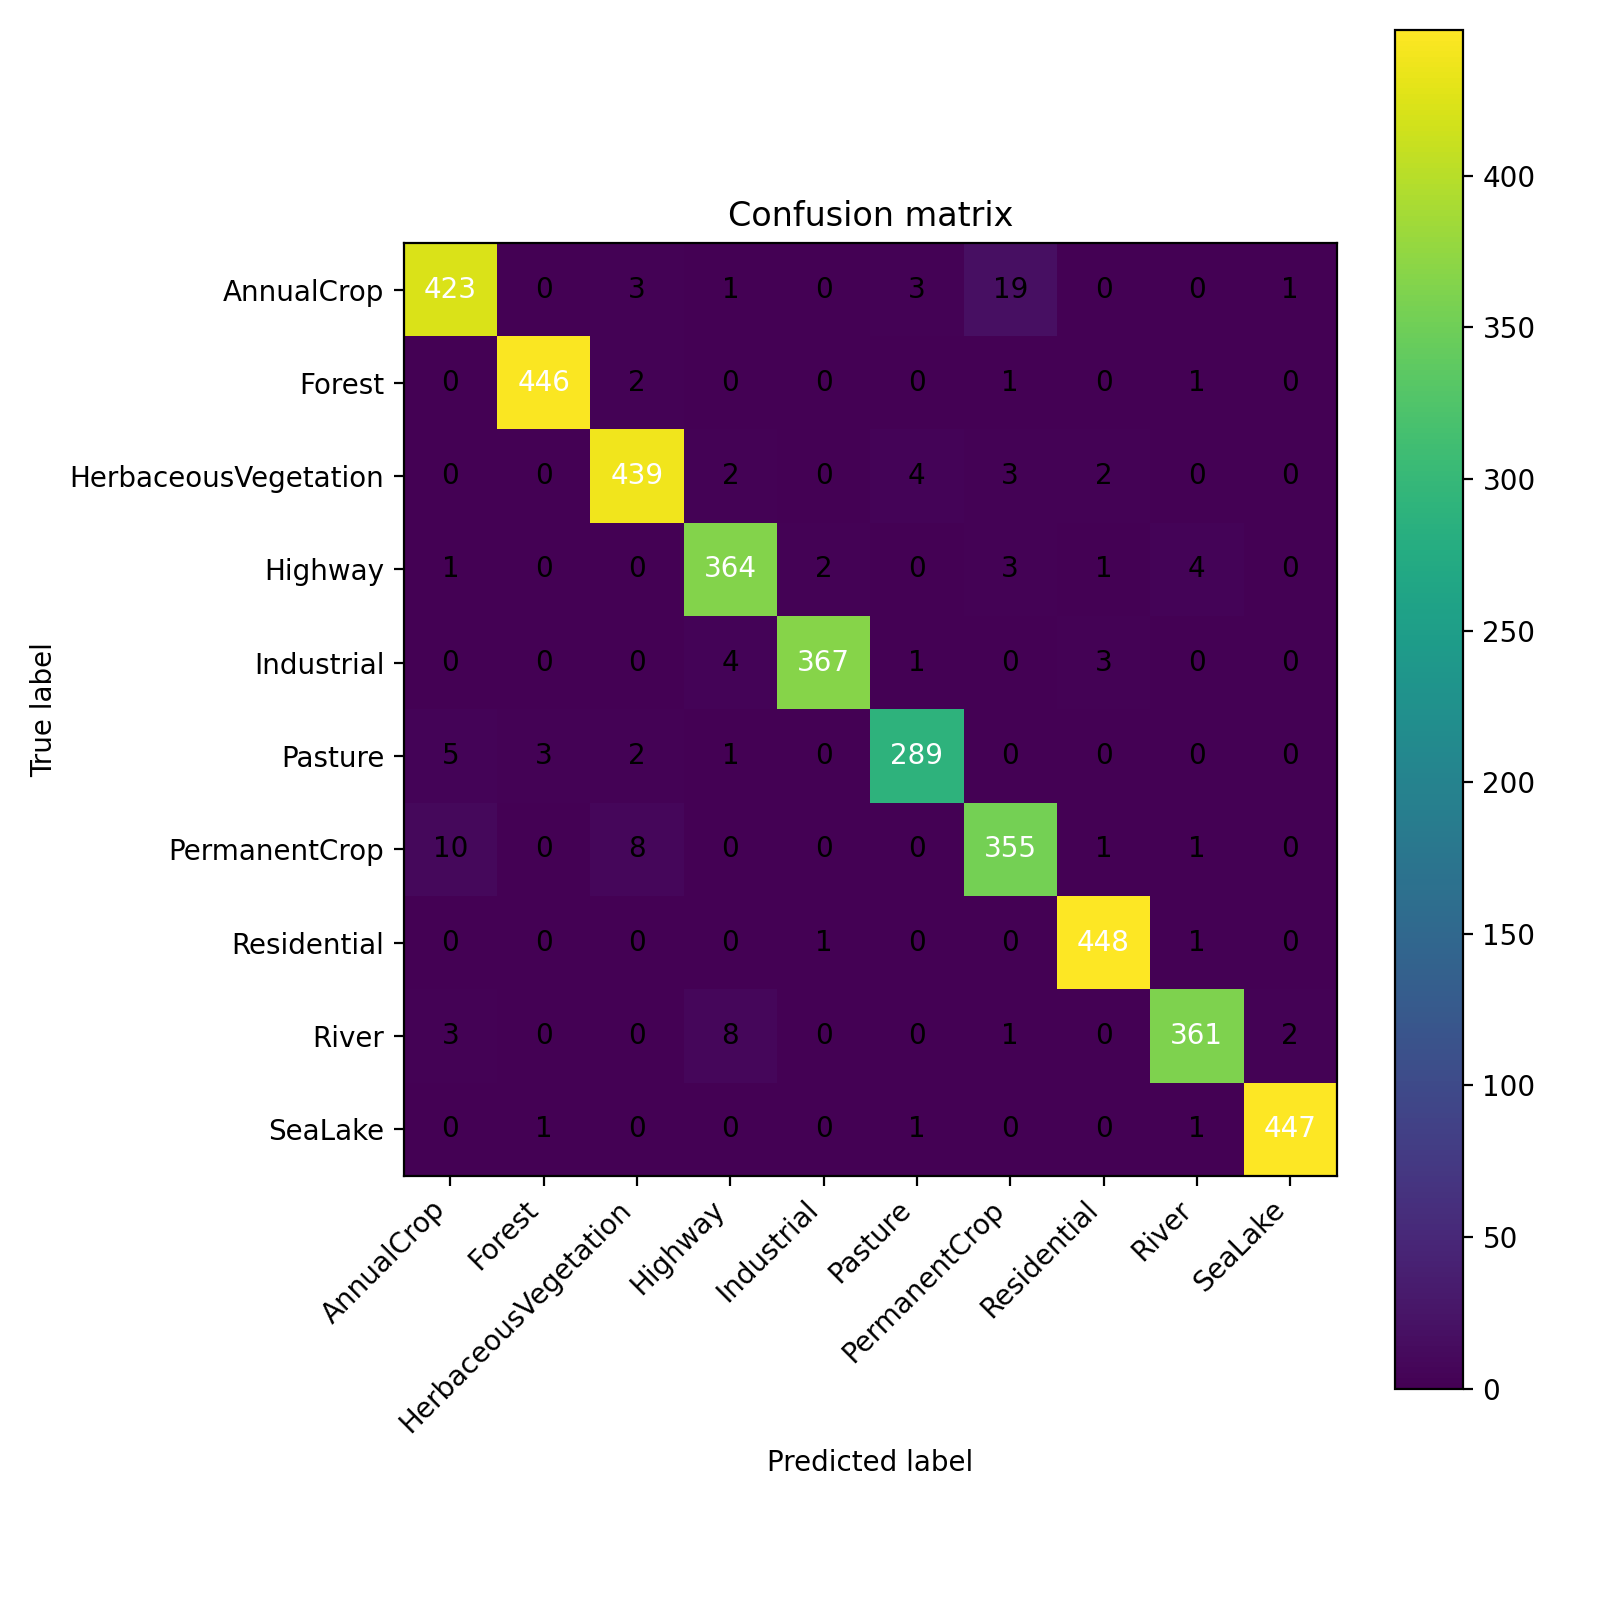
\includegraphics[width=0.70\textwidth]{figures/efficientnet_b0/multiclass_confusion_matrix.png}
    \caption{Confusion matrix of the EfficientNet-B0 model on the 10-class test split.}
    \label{fig:efficientnet_multiclass_cm}
\end{figure}

Figure~\ref{fig:efficientnet_binary_curves} shows the loss and accuracy curves for the binary vegetation classification task. The validation performance improves over the full training run, and the best checkpoint was selected in epoch 29.

\begin{figure}[H]
    \centering
    \begin{minipage}{0.48\textwidth}
        \centering
        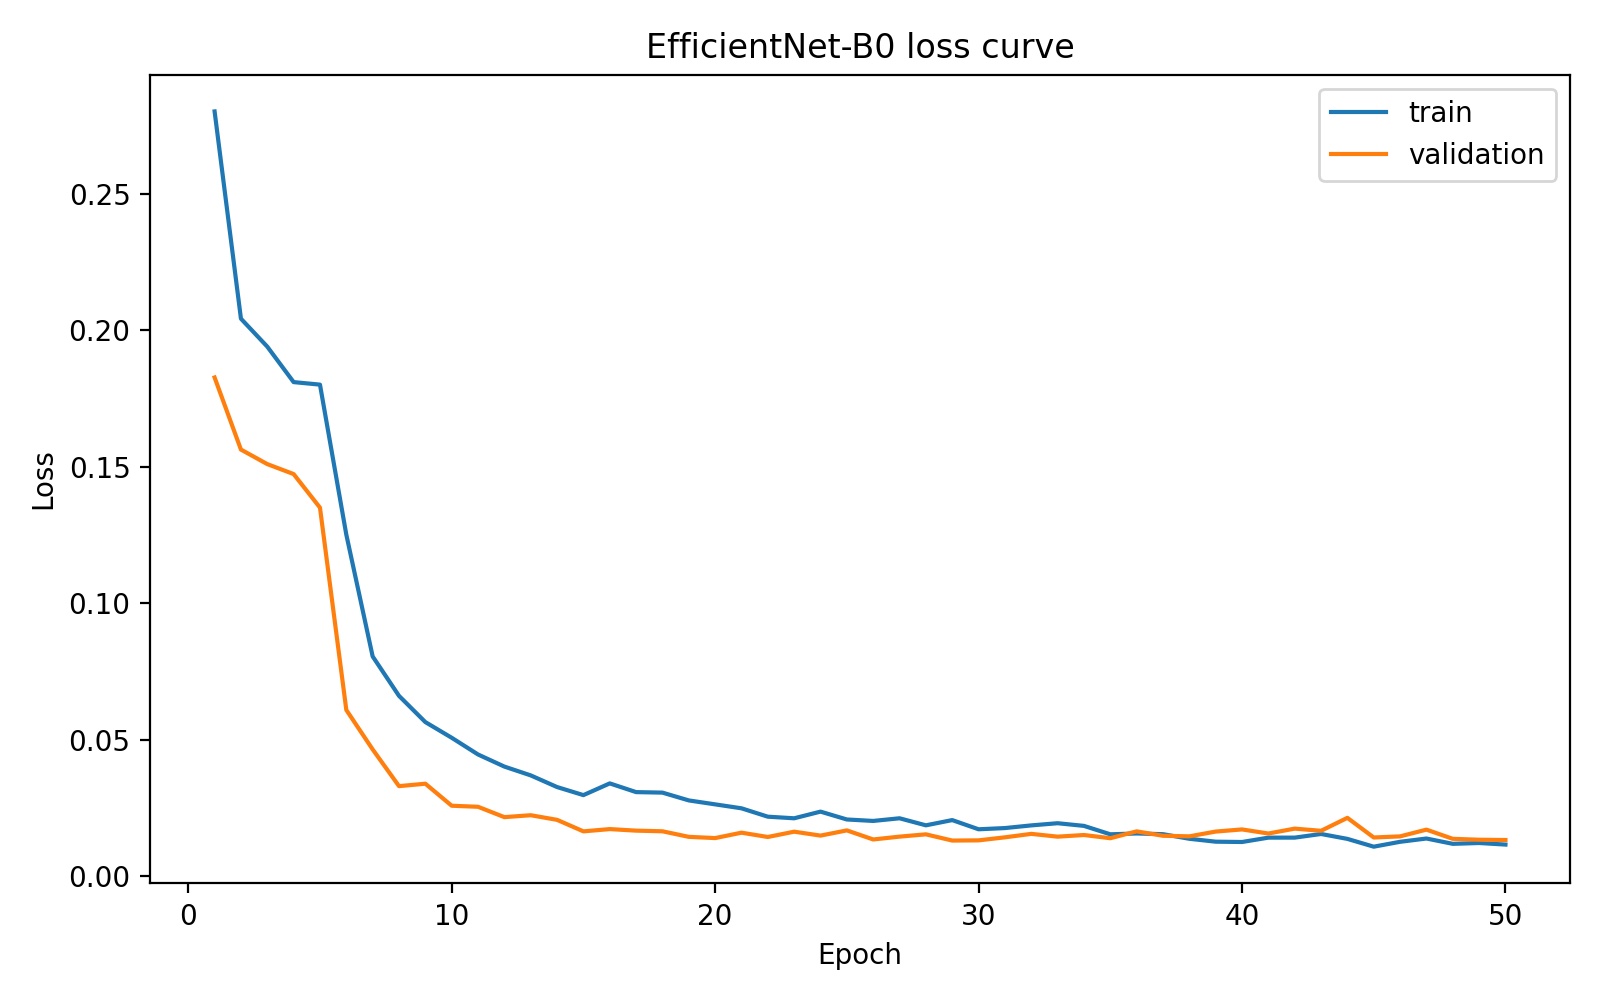
\includegraphics[width=\linewidth]{figures/efficientnet_b0/binary_loss_curve.png}
    \end{minipage}
    \hfill
    \begin{minipage}{0.48\textwidth}
        \centering
        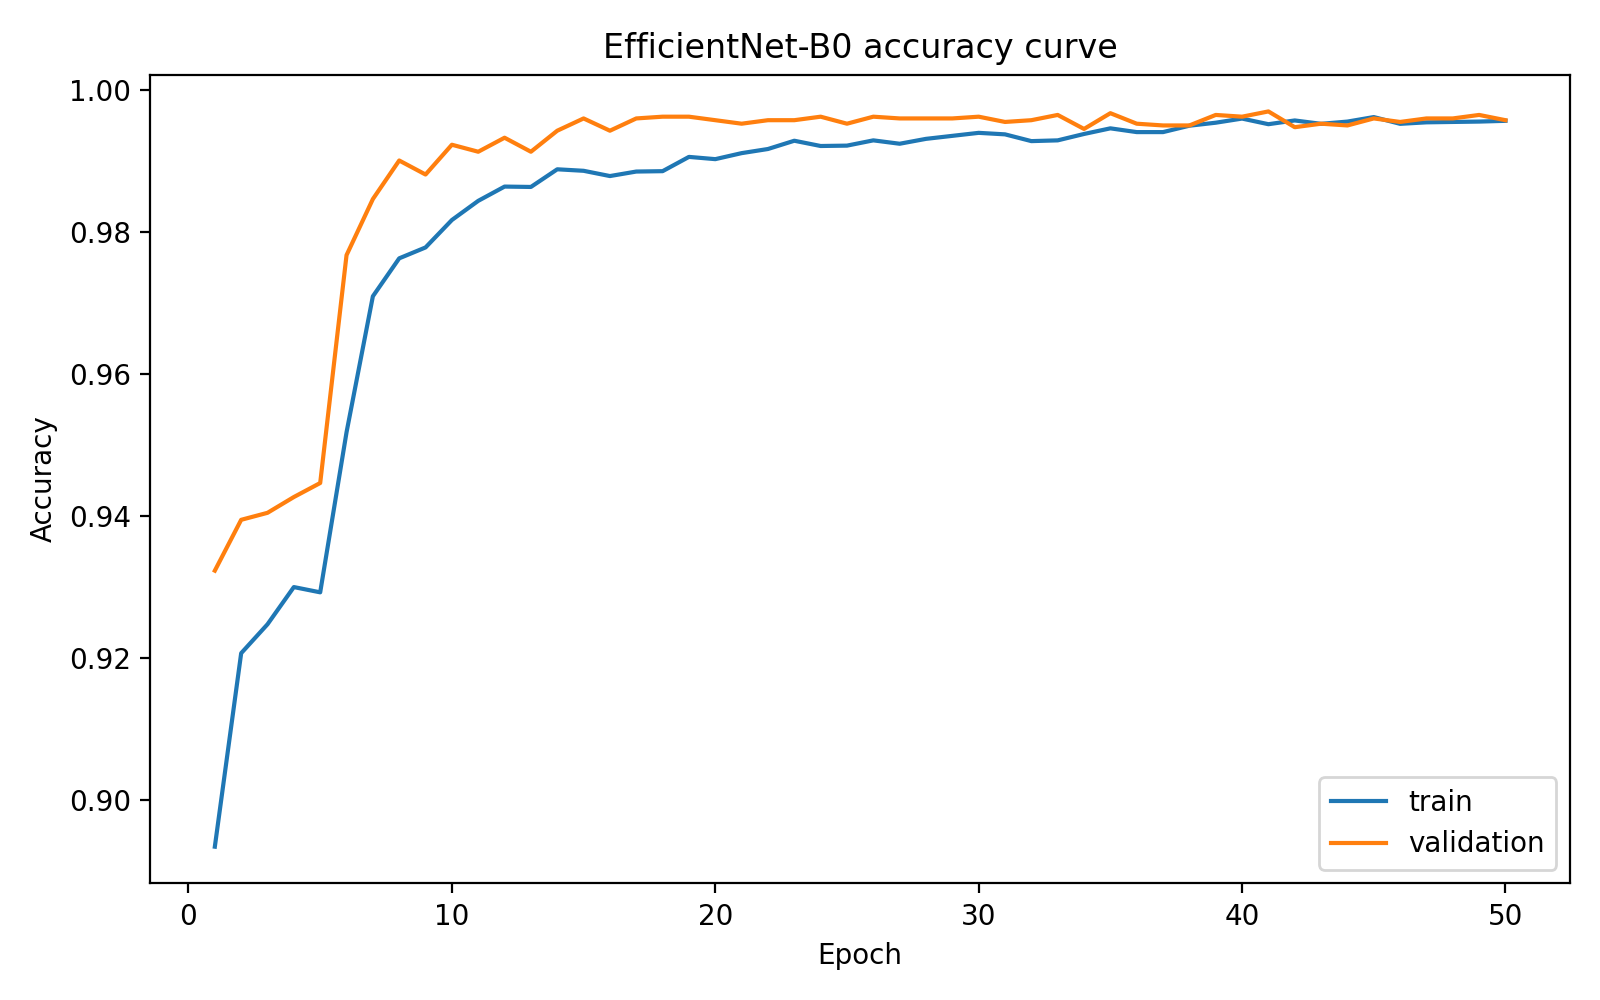
\includegraphics[width=\linewidth]{figures/efficientnet_b0/binary_accuracy_curve.png}
    \end{minipage}
    \caption{Loss and accuracy curves of the EfficientNet-B0 model on the binary task.}
    \label{fig:efficientnet_binary_curves}
\end{figure}

Figure~\ref{fig:efficientnet_binary_cm} shows the confusion matrix for the binary test split. The binary task produces fewer errors than the 10-class task because several visually similar vegetation classes are grouped into one shared class.

\begin{figure}[H]
    \centering
    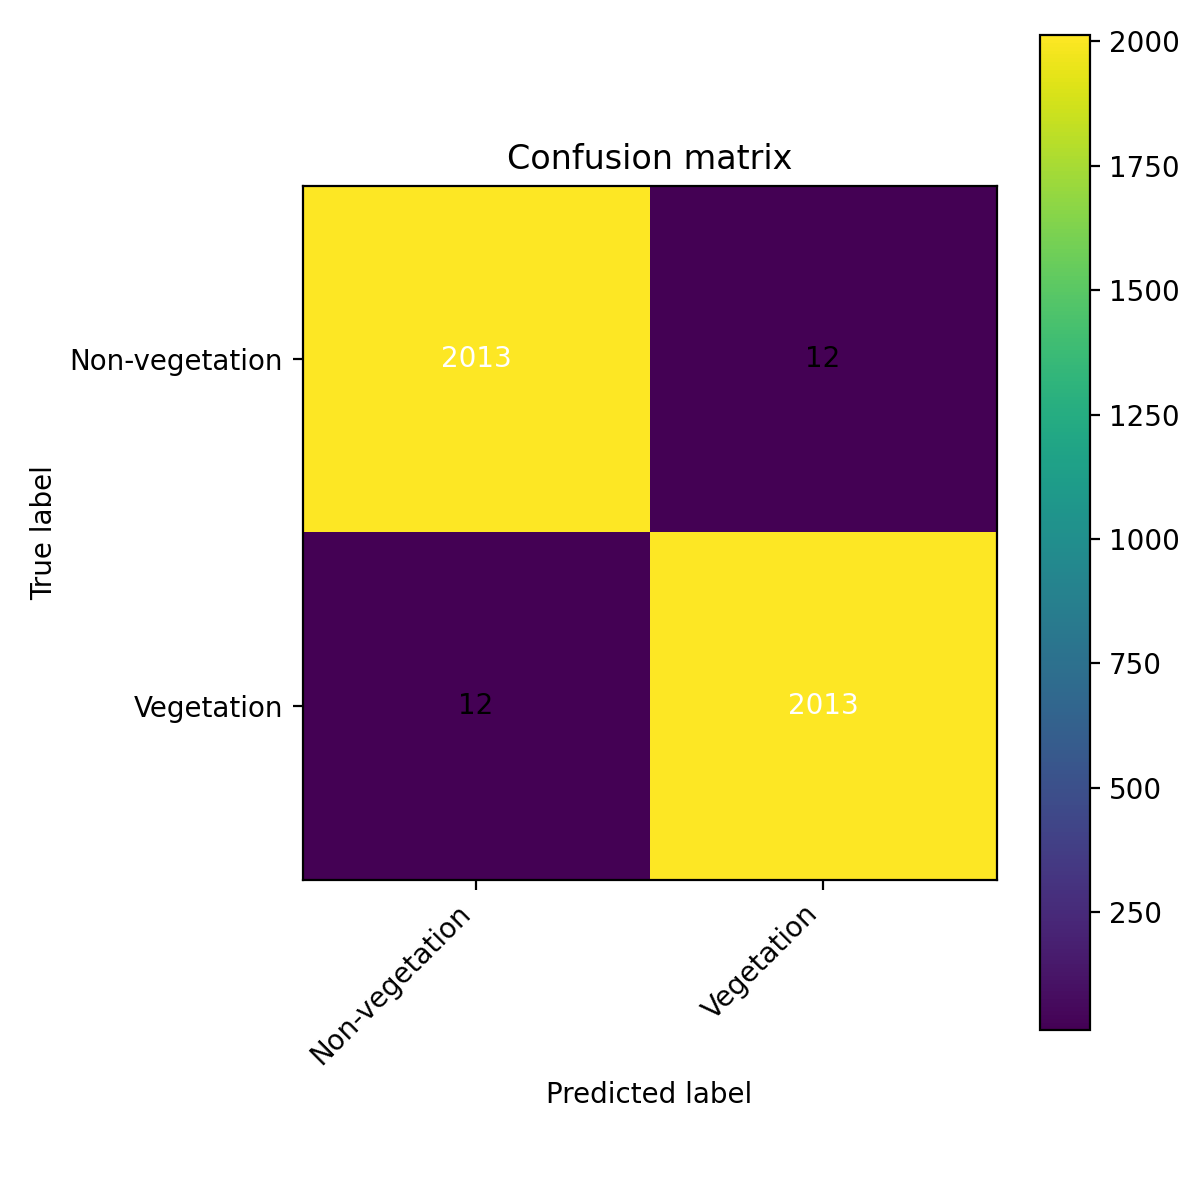
\includegraphics[width=0.60\textwidth]{figures/efficientnet_b0/binary_confusion_matrix.png}
    \caption{Confusion matrix of the EfficientNet-B0 model on the binary test split.}
    \label{fig:efficientnet_binary_cm}
\end{figure}

The 10-class model reached a test accuracy of 0.9726 and a test macro-F1 of
0.9719. This means that 3939 out of 4050 test images were classified correctly.
The epoch-46 checkpoint was used as the final model, based on the lowest
validation loss.

The binary task reached a test accuracy and macro-F1 of 0.9941. This means that
4026 out of 4050 test images were classified correctly. The binary task is
again easier than the full 10-class task, because visually similar vegetation
classes are grouped together.
